The data for this lab came from a HPGe detector collected by Dr. Ross Barnowski. The sources used to generate the spectrum are shown in Table 1.

\begin{table}[]
\centering
\caption{Sources for Lab0}
\label{my-label}
\begin{tabular}{|l|l|l|l|l|}
\hline
$^{241}$Am & $^{133}$Ba & $^{60}$Co & $^{137}$Cs & $^{137}$Cs \\ \hline
\end{tabular}
\end{table}

The energy calibration was performed using a two-point linear fit between $^{137}$Cs and $^{241}$Am. To perform the calibration, a simple python program searched the raw spectrum data of $^{137}$Cs and $^{241}$Am looking for the largest peaks within the spectrum. The program iterated over the spectrum by channel trying to identify a large delta (40000) in the counts. Because $^{137}$Cs and $^{241}$Am have single gamma ray photopeaks, a large delta ensures no other noise in the signal could be misconstrued as photopeaks. The identified photopeaks of $^{137}$Cs and $^{241}$Am are depicted in Figure \ref{Peaks}.

\begin{figure}[H]
\centering
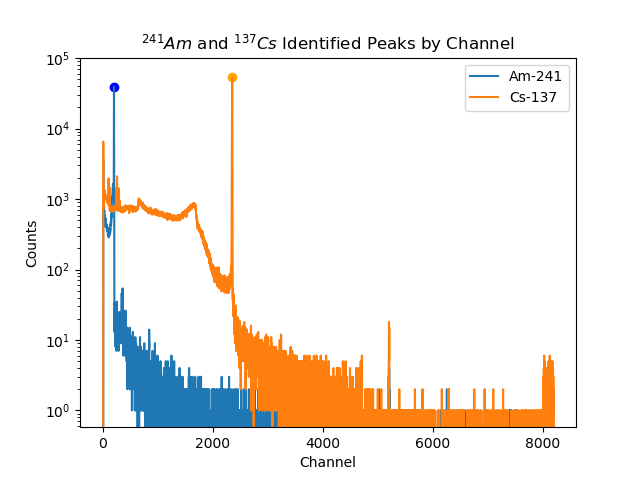
\includegraphics[scale=0.8]{images/Peaks.png}
\caption{Photopeaks of $^{137}$Cs and $^{241}$Am}
\label{Peaks}
\end{figure}

Once the $^{137}$Cs and $^{241}$Am peaks were discovered, the python function polyfit was used to plot a linear line. The inputs for polyfit were the channel of the peak and the actual gamma-ray photopeak energy as listed in the IAEA Isotope Browser. The polyfit output was a slope and intercept that can be used to translate channel to energy. Lastly, the polyfit "calibrated" energy was applied to the $^{133}$Ba spectra.
